%%%%%%%%%%%%%%%%%%%%%%%%%%%%%%%%%%%%%%%%%%%%%%%%%%%%%%%%%%%%%%%%%%%%%%
% How to use writeLaTeX:
%
% You edit the source code here on the left, and the preview on the
% right shows you the result within a few seconds.
%
% Bookmark this page and share the URL with your co-authors. They can
% edit at the same time!
%
% You can upload figures, bibliographies, custom classes and
% styles using the files menu.
%
% If you're new to LaTeX, the wikibook is a great place to start:
% http://en.wikibooks.org/wiki/LaTeX
%
%%%%%%%%%%%%%%%%%%%%%%%%%%%%%%%%%%%%%%%%%%%%%%%%%%%%%%%%%%%%%%%%%%%%%%
\documentclass{tufte-handout}

%\geometry{showframe}% for debugging purposes -- displays the margins

\usepackage{amsmath}

% Set up the images/graphics package
\usepackage{graphicx}
\setkeys{Gin}{width=\linewidth,totalheight=\textheight,keepaspectratio}
\graphicspath{{graphics/}}

\title{Stata Lab 4: Randomization}
\author{DIME Analytics \\ dimeanalytics@worldbank.org}
% \date{24 January 2009}  % if the \date{} command is left out, the current date will be used

% The following package makes prettier tables.  We're all about the bling!
\usepackage{booktabs}

% The units package provides nice, non-stacked fractions and better spacing
% for units.
\usepackage{units}

% The fancyvrb package lets us customize the formatting of verbatim
% environments.  We use a slightly smaller font.
\usepackage{upquote}
\usepackage{fancyvrb}
\fvset{fontsize=\normalsize}
\renewcommand{\FancyVerbFormatLine}{\color{violet}}
\DefineShortVerb{\|}

% Small sections of multiple columns
\usepackage{multicol}

% Provides paragraphs of dummy text
\usepackage{lipsum}

% These commands are used to pretty-print LaTeX commands
\newcommand{\doccmd}[1]{\texttt{\textbackslash#1}}% command name -- adds backslash automatically
\newcommand{\docopt}[1]{\ensuremath{\langle}\textrm{\textit{#1}}\ensuremath{\rangle}}% optional command argument
\newcommand{\docarg}[1]{\textrm{\textit{#1}}}% (required) command argument
\newenvironment{docspec}{\begin{quote}\noindent}{\end{quote}}% command specification environment
\newcommand{\docenv}[1]{\textsf{#1}}% environment name
\newcommand{\docpkg}[1]{\texttt{#1}}% package name
\newcommand{\doccls}[1]{\texttt{#1}}% document class name
\newcommand{\docclsopt}[1]{\texttt{#1}}% document class option name

\begin{document}

\maketitle% this prints the handout title, author, and date

\begin{marginfigure}%
  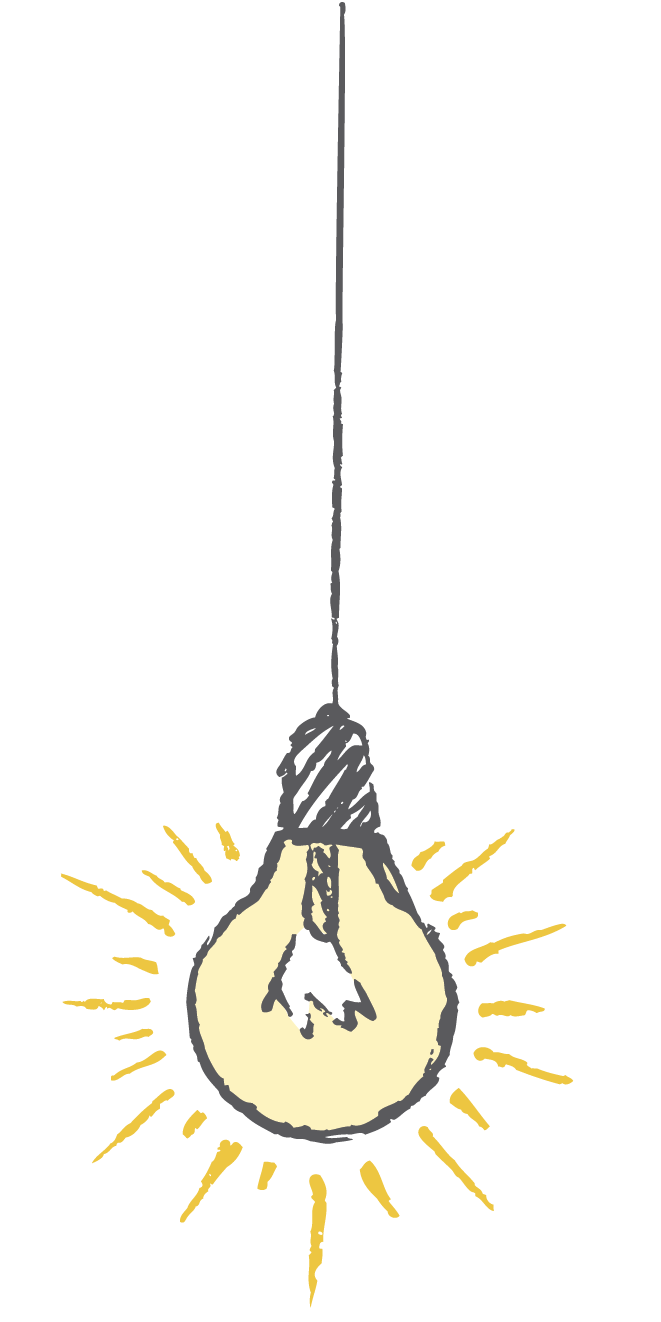
\includegraphics[width=\linewidth]{light.png}
\end{marginfigure}

\begin{abstract}
In this lab, we will practice defining replicable randomization
and running simple randomization as well as
common randomization procedures we have covered during the session.

\bigskip\noindent \textbf{Exercise Objectives}:
\begin{enumerate}
  \item Define three rules of replicable randomization using Stata
  \item Learn how to conduct simple-design randomization
  \item Use the |randtreat| command to handle common randomizations
\end{enumerate}

\bigskip\noindent \textbf{Getting Started}:
\begin{enumerate}
 \item Open your |/DataWork/| folder for the full training. It should have subfolders for each of the Labs; if it does not, use |iefolder| to create the folder |/Lab4/| now.
 \item You will find a data file that we created in Lab 2, |hh_roster.dta| in the public Field Coordinator Training folder. Save this dataset to |/DataWork/Lab4/|.
\end{enumerate}
\end{abstract}

%\printclassoptions
\section{The three rules of replicable randomization}

To make randomization replicable, we need to follow three rules:
same Stata version, same seed, and data ordered the same way.
In this section, we will write code to satisfy those rules.
These must be done at the beginning of any dofile that invokes randomization
for any reason, or it won’t produce the same results each time it is run.
The best practice is to do as few randomizations as possible in each dofile,
and set these keys at the beginning of every one.

\subsection{Set the software version}

Notice that the |Project_MasterDofile.do| includes |ieboilstart| as shown:
\begin{Verbatim}
  ieboilstart, version(12.1)
  `r(version)'
\end{Verbatim}
You must use this command before opening a dataset or defining programs.
|ieboilstart| sets a lot of settings,
some of which require that you have no data loaded in Stata.\sidenote{\url{https://dimewiki.worldbank.org/wiki/ieboilstart}}
The part of this command we are interested in today is
to set Stata to a certain “version”,
which is the first requirement of replicable randomization.
This is because different versions of Stata use different randomization algorithms.
You might already know the |version| command to do so,
\textit{and you will still need to include it in individual dofiles},
but we will also use |ieboilstart| since it prepares
other useful Stata settings, like the maximum number of variables, simultaneously.

\marginnote{One important setting you might not be used to is \texttt{set varabbrev off}.
This prevents you from referring to variable names by abbreviations,
such as referring to \texttt{\_merge} as \texttt{\_m}.
This is good practice because it prevents Stata from changing the interpretation
of your code if the dataset changes in specific ways.}

Unless you really need, always use an older version
of Stata so people with older version of Stata can also use it.
If you set Stata to a newer
version, other users with older Stata cannot run your code.
Therefore, start your dofile with |version 12.1|, and
type |di c(version)| to confirm the |version| setting is now |12.1|.
If you have followed the steps above,
then you have satisfied the first rule of replicable randomization.

\subsection{Set the randomization seed}

Now you should understand and implement the |set seed| command.
Stata draws ``pseudo-random'' numbers
(meaning they are as good as random but not actually random),
and the seed determines where in this list Stata will start from.
This is one of the critical differences between Stata versions,
and why the version must be set first.
It is good practice to use a random number as your seed
each time you write a randomization dofile. Do this now:
\begin{enumerate}
  \item Start a new dofile in |/Lab4/|. Call it |/Lab4/randomization-1.do|.
  \item Choose a random six-digit number. For example,
  use the website \url{https://www.random.org} to generate a six-digit seed,
  or use the shortcut \url{https://bit.ly/stata-random}.
  If you don't have access to the internet,
  you can take a banknote from your wallet and
  use the last six digits of the serial number.
  Do not use the six first digits as
  they tend to be similar across banknotes in most currencies.
  \item Write |set seed| in the code and
  use a comment to document how you obtained the random number.
\end{enumerate}
If you do this properly, you will have satisfied the
second rule of replicable randomization.

\subsection{Uniquely order the dataset}

Now, |use| and |sort| the |hh_roster.dta| data set
in a unique and unchangeable way.
Use the command |isid, sort| on a variable that you are sure will never change:
in this case, the unique identifiers should be |hh_id mem_id|.
You must also make sure the dataset itself will not change,
or the randomization will, too!
If you do this properly you have taken care of the
third rule of replicable randomization.

\section{A simple randomization}

Now, let’s practice randomization.
This demo dataset already has a |treatment| variable in it: |drop| it.
First, we will produce a two-group “equal probability”
randomization at the individual level. To do this, follow these steps:
\begin{enumerate}
  \item Draw a pseudorandom number for every observation with:
\begin{Verbatim}
  gen random = runiform(0,1)
\end{Verbatim}
  \item Use |histogram random| to confirm that this worked.
  \item Split the sample into two equal-sized group with |xtile|.
  Note that you could create as many groups as you like. Write:
\begin{Verbatim}
  xtile group = random, n(2)
\end{Verbatim}
  \item Next, generate the treatment variable using |recode|, including the  labelling function:
\begin{Verbatim}
  recode group (1=0 "Control")(2=1 "Treatment")) , gen(treatment)
\end{Verbatim}
  \item Use |tab treatment| to confirm that the groups are equally-sized.
  \item If you want to be sure you did this right, you can use a rank-sum test.
  You want a high p-value showing that |treatment| is
  totally uncorrelated with the sort order of the data. Write:
\begin{Verbatim}
  gen n = _n
  ranksum n , by(treatment)
\end{Verbatim}
  \item Now, |drop| all the variables you don’t need: |random|, |group|, and |n|.
  \item Save this data as |hh_roster_randomized.dta|.
\end{enumerate}

In the next steps, we will confirm that your randomization is exactly replicable.
Starting from the next line in the dofile,
write a new section that repeats the randomization \textit{exactly}.
Do not |save| the dataset once you have re-created the treatment assignment.
Instead, write:
\begin{Verbatim}
  cf _all using "${Lab5}/hh_roster_randomized.dta"
\end{Verbatim}
The |cf| command (``compare file'') tells you if the variables in the open dataset
are exactly the same as the ones in the |using| file.
If you have done this right,
the current dataset will match exactly the one you have
already saved, and the |cf| command will run without any errors or outputs.
If not, try to find out why!
This is a great confirmation that you have randomized replicably.

\section{Complex randomization}

In this section, we will continue working on the same data set
we used in the previous section,
but will try different randomization design –
multiple treatment arms, unequal group size,
indivisible sample size and stratification.
We will use the |randtreat| command for the complex designs we will cover
in this section and you should feel free to use that in practice.

\subsection{Multiple treatment arms}

Suppose you need to assign this sample (4,317 individuals) equally
to one control group and four different treatment groups with equal size.
Duplicate, then modify the do-file you wrote in the previous section
to accomplish this as |randomization-2.do|.
Did you get five equally big groups?
(Note that the |ranksum| check no longer works.)
There should be one group with one more observation 4317/5 = 863
with two left over. Since we assigned treatment randomly,
was it randomly decided which group gets an extra observation?
Change the seed a couple of times and re-run your code. Does it change?

It is not random which group gets the extra observation,
but it is random which observation that is that extra observation.
In this example, it does not matter too much as there is only
a difference of one observation between very large groups.
But let’s think about a stratified example
(when we split the sample up in many subsamples, then randomize).
It could be the case that in each of those subsamples
it is the same group that gets the extra observation (which we call “misfits”).
Then we start to have a bigger and bigger size imbalance
as that group gets one extra observation per stratum.
To manually code up a solution to this
is a much bigger challenge than what one might first think.

|randtreat| is a user-written Stata command
which can correctly solve this issue
as well as other issues we will go over in this section.
We will practice how to use the command
to handle the issues in complex randomization design. To get started:
\begin{enumerate}
  \item Install |randtreat| by writing |ssc install randtreat|
  \item Type |help randtreat|. Read the syntax and description
  to understand what you can do with the command.
  \item Run |randtreat| command the |multiple| option
  to randomly assign the sample into four different groups.
  Tabulate the treatment variable to see how students were assigned.
  Note that the misfit observation will be recorded as missing (ie, in no group).
  \item Run the same code above,
  but include the |misfits| option. Since we have not covered
  stratified randomization yet, use |global| as a method of treating misfits.
  \item Tabulate the treatment variable. To which group were misfits assigned?
  \item Generate a few more |treatment| variables with the same code,
  then tabulate those variables. To which groups were misfits assigned?
  Was it random?
\end{enumerate}

\subsection{Unequal treatment arms}

Suppose you want to randomly assign 40\% of your sample
to a control group and 60\% to a treatment group.
Duplicate, then modify the do-file you wrote
in the first section to accomplish this as |randomization-3.do|.
First, randomize individuals using the |xtile| method
as we did in the original simple randomization.
How should you modify your code to do so?
Then, randomize individuals using the |randtreat| command.
You need to use the |unequal| option to do so.
Tabulate the treatment variable you generated
to confirm students were randomly assigned to unequal groups.

\subsection{Clustered and stratified randomization}

In clustered randomizations, we have a listing of, say, individuals,
but for practical reasons we can only assign treatments at the household level.
Assume that this is the case for this dataset,
and produce a 50-50 equal-probability clustered randomization
at the household level
such that all members of each household are in the same group.
(Hint: use the |tag_hh| variable;
it may be conceptually easier to use |keep| and |merge| strategically.)

In stratified randomization,
we first select variables of interest
and divide the sample into sublists (strata) based on the selected variables.
Units are randomized \textit{within} each stratum.
We use stratified randomization to achieve balance on major covariates.
Do this using the district indicator |hh_id_09| in this dataset,
while clustering by household.
This should give you a randomization such that
(A) each \textit{district} has a 50-50 split
between treatment and control at the household level;
and (B) each household has the same treatment assignment for all members.
We can easily stratify via the |randtreat| command,
but you will still have to re-use the manual clustering technique you implemented above.
Duplicate, then modify the do-file you wrote in the first section to accomplish these tasks as |randomization-4|.do.

Thanks to the template creators.\cite{tuftelatex}

\bibliography{sample-handout}
\bibliographystyle{plainnat}

\newpage

\begin{figure*}[h]
{\setstretch{0.7}
\VerbatimInput[frame=lines,numbers=left,label=randomization-1.do]
{../DataWork/Lab4/randomization-1.do}}
\end{figure*}

\begin{figure*}[h]
{\setstretch{0.7}
\VerbatimInput[frame=lines,numbers=left,label=randomization-2.do]
{../DataWork/Lab4/randomization-2.do}}
\end{figure*}

\begin{figure*}[h]
{\setstretch{0.7}
\VerbatimInput[frame=lines,numbers=left,label=randomization-3.do]
{../DataWork/Lab4/randomization-3.do}}
\end{figure*}

\begin{figure*}[h]
{\setstretch{0.7}
\VerbatimInput[frame=lines,numbers=left,label=randomization-4.do]
{../DataWork/Lab4/randomization-4.do}}
\end{figure*}

\end{document}
